%% Template for Stata-Journal Quarto manuscript

%% Main

% main.tex - a driver for your Stata Journal insert
% This file should only be changed according to the AUTHOR notes below.
% The Stata Press document class

\documentclass[bib]{statapress}

% Page dimensions
\usepackage[crop,newcenter,frame]{pagedims}
% The Stata Journal styles
\usepackage{sj}
% Stata Log listings and useful macros
\usepackage{stata}
% Encapsulated PostScript figures
\usepackage{epsfig}
% Shadow package to render technical note figure
\usepackage{shadow}
\usepackage{amsmath,amssymb} 
% EDITORS: volume number, issue number, month, and year
\usepackage{setspace}
%% Hide Links
%CodeThis is for Executed code. But may not be necessary
\usepackage{color}
\usepackage{fancyvrb}
\newcommand{\VerbBar}{|}
\newcommand{\VERB}{\Verb[commandchars=\\\{\}]}
\DefineVerbatimEnvironment{Highlighting}{Verbatim}{commandchars=\\\{\}}
% Add ',fontsize=\small' for more characters per line
\usepackage{framed}
\definecolor{shadecolor}{RGB}{255,255,255}
\newenvironment{Shaded}{\begin{snugshade}}{\end{snugshade}}
\newcommand{\KeywordTok}[1]{\textcolor[rgb]{0.00,0.0,0.0}{#1}}
\newcommand{\NormalTok}[1]{\textcolor[rgb]{0.00,0.0,0.0}{#1}}




%% Ref

 

\sjsetissue{vv}{ii}{mm}{yyyy}

%%%%%%%%%%%%%%%%%%%%%%%%%%%%%%%%%%%%%%%%%%%%%%%%%%%%%%%%%%%%%%%%%%%%%%%%%%%%%%%


\providecommand{\tightlist}{%
  \setlength{\itemsep}{0pt}\setlength{\parskip}{0pt}}\usepackage{longtable,booktabs,array}
\usepackage{calc} % for calculating minipage widths
% Correct order of tables after \paragraph or \subparagraph
\usepackage{etoolbox}
\makeatletter
\patchcmd\longtable{\par}{\if@noskipsec\mbox{}\fi\par}{}{}
\makeatother
% Allow footnotes in longtable head/foot
\IfFileExists{footnotehyper.sty}{\usepackage{footnotehyper}}{\usepackage{footnote}}
\makesavenoteenv{longtable}
\usepackage{graphicx}
\makeatletter
\def\maxwidth{\ifdim\Gin@nat@width>\linewidth\linewidth\else\Gin@nat@width\fi}
\def\maxheight{\ifdim\Gin@nat@height>\textheight\textheight\else\Gin@nat@height\fi}
\makeatother
% Scale images if necessary, so that they will not overflow the page
% margins by default, and it is still possible to overwrite the defaults
% using explicit options in \includegraphics[width, height, ...]{}
\setkeys{Gin}{width=\maxwidth,height=\maxheight,keepaspectratio}
% Set default figure placement to htbp
\makeatletter
\def\fps@figure{htbp}
\makeatother

\makeatletter
\@ifpackageloaded{caption}{}{\usepackage{caption}}
\AtBeginDocument{%
\ifdefined\contentsname
  \renewcommand*\contentsname{Table of contents}
\else
  \newcommand\contentsname{Table of contents}
\fi
\ifdefined\listfigurename
  \renewcommand*\listfigurename{List of Figures}
\else
  \newcommand\listfigurename{List of Figures}
\fi
\ifdefined\listtablename
  \renewcommand*\listtablename{List of Tables}
\else
  \newcommand\listtablename{List of Tables}
\fi
\ifdefined\figurename
  \renewcommand*\figurename{Figure}
\else
  \newcommand\figurename{Figure}
\fi
\ifdefined\tablename
  \renewcommand*\tablename{Table}
\else
  \newcommand\tablename{Table}
\fi
}
\@ifpackageloaded{float}{}{\usepackage{float}}
\floatstyle{ruled}
\@ifundefined{c@chapter}{\newfloat{codelisting}{h}{lop}}{\newfloat{codelisting}{h}{lop}[chapter]}
\floatname{codelisting}{Listing}
\newcommand*\listoflistings{\listof{codelisting}{List of Listings}}
\makeatother
\makeatletter
\makeatother
\makeatletter
\@ifpackageloaded{caption}{}{\usepackage{caption}}
\@ifpackageloaded{subcaption}{}{\usepackage{subcaption}}
\makeatother
\begin{document}

%% AUTHOR:  Include your article here.

%% TITLE

 
\title[QRegressions FE]{Estimation of Quantile Regressions with Multiple
Fixed Effects}


\makeatletter

\inserttype[st0001]{article}
\author{Rios-Avila, Siles, Canavire-Bacarreza}{
Fernando Rios-Avila\\
Levy Economics Institute\\Annandale-on-Hudson, NY\\
\href{mailto:friosavi@levy.org}{friosavi@levy.org}
\and 
Leonardo Siles\\
Universidad de Chile\\Santiago, Chile\\
\href{mailto:lsiles@fen.uchile.cl}{lsiles@fen.uchile.cl}
\and 
Gustavo Canavire-Bacarreza\\
The World Bank\\Washington, DC\\
\href{mailto:gcanavire@worldbank.org}{gcanavire@worldbank.org}
}
 
 
 

\maketitle

\begin{abstract}

This paper introduces two new Stata commands, \texttt{qregfe} and
\texttt{qregplot}, designed for estimating and visualizing quantile
regression models with fixed effects. \texttt{qregfe} implements several
methodologies including Correlated Random Effects, Canay (2011), a
modified Canay estimator, and Method of Moments Quantile Regression
(Machado and Santos Silva, 2019). This allows researchers to control for
unobserved heterogeneity in panel data settings while examining
heterogeneous effects across the conditional distribution.
\texttt{qregplot} facilitates visualization of quantile regression
results, enabling graphical examination of covariate effects across
different quantiles.

\keywords{\inserttag, Quantile Regression, Fixed Effects, Panel Data}
\end{abstract}

\section{Introduction}\label{sec-intro}

Quantile regression, introduced by \citet{koenker1978}, has become an
important tool in economic analysis, allowing researchers to examine how
the relationship between the dependent and independent variables varies
across different points of the conditional distribution of the outcome.
While ordinary least squares focuses on analyzing the conditional mean,
quantile regression provides a more comprehensive view of how covariates
impact the entire conditional distribution of the dependent variable.
This can reveal heterogeneous effects that may be otherwise overlooked
when analyzing the conditional mean.

A relatively recent development in the literature has focused on
extending quantile regression analysis in a panel data setting to
account for unobserved, but time-fixed heterogeneity. This is
particularly important in empirical research, where unobserved
heterogeneity can bias estimates of the effects of interest. However, as
is common in the estimation of non-linear models with fixed effects,
introducing fixed effects in quantile regression models poses several
challenges. On the one hand, the simple inclusion of fixed effects can
lead to an incidental parameter problem, which can bias estimates of the
quantile coefficients \citep{neymanscott1948, lancaster2000}. On the
other hand, the computational complexity of estimating quantile
regression models with fixed effects can be prohibitive, particularly
for large datasets with multiple high-dimensional fixed effects. While
many strategies have been proposed for estimating this type of model
(see \citet{galvao2017quantile} for a review), none has become standard
due to restrictive assumptions regarding the inclusion of fixed effects
and the computational complexity.

In spite of the growing interest in estimating quantile regression
models with fixed effects in applied research, particularly in the
fields of labor economics, health economics, and public policy, among
others, there are few commands that allow the estimation of such models.
In Stata, there are three main built-in commands available for
estimating quantile regression: \texttt{qreg}, \texttt{ivqregress}, and
\texttt{bayes:\ qreg}, and none of them allow for the inclusion of fixed
effects, other than using the dummy variable approach. From the
community-contributed commands, there is \texttt{xtqreg}, which
implements a quantile regression model with fixed effects based on the
method of moments proposed by \citet{mss2019}, and more recently
\texttt{xtmdqr} which implements a minimum distance estimation of
quantile regression models with fixed effects described in
\citet{melly2023}. In both cases, these commands are constrained to a
single set of fixed effects.\footnote{There are other
  community-contributed commands like \texttt{xtrifreg},
  \texttt{rifhdfe}, \texttt{qregpd}, \texttt{rqr} among others that
  allow for the estimation of quantile regression models, but do not
  estimate conditional quantile regressions, but instead focus on
  unconditional quantile regressions, or quantile treatment effects.}

To address this, in this paper we introduce a new Stata command for
estimating quantile regressions with multiple fixed effects:
\texttt{qregfe}. This command implements: the extended estimator of
quantile regression via moments (\texttt{mmqreg}) proposed by
\citet{mss2019} and \citet{riosavila2024}; an implementation of a
correlated random effects estimator based on \citet{abrevaya2008},
\citet{wooldridge2019} and \citet[Ch12.10.3]{wooldridge2010}; the
estimator proposed by \citet{canay2011}, and a proposed modification of
this approach. In addition, we also present an auxiliary command
\texttt{qregplot} for the visualization of the quantile regression
models.

This command offers the advantage of allowing for the estimation of
conditional quantile regressions while controlling for multiple fixed
effects. First, they leverage existing Stata commands, as well as other
community-contributed commands, to allow users to estimate quantile
regression models and their standard errors under different assumptions.
Second, they reduce the impact of the incidental parameters problem
depending on the assumptions underlying the data generating process. In
terms of standard errors, \texttt{mmqreg} allows for the estimation of
analytical standard errors (see \citet{mss2019} and
\citet{riosavila2024}), whereas \texttt{qregfe} emphasizes the use of
bootstrap standard errors. Finally, the command is designed to be
user-friendly, allowing for the estimation of quantile regression models
with fixed effects in a single line of code.

The remainder of the paper is organized as follows. Section 2 reviews
the methodological framework for quantile regression, along with the
methods and formulas behind the estimators implemented by
\texttt{qregfe} command. Section 3 introduces the commands, along with a
brief description of their syntax and options. Section 4 introduces an
auxiliary command for the visualization of quantile regression models.
Section 6 provides an empirical application demonstrating their use.
Section 7 concludes.

\section{The Basics}\label{sec-basics}

Quantile regressions allow researchers to identify the heterogeneous
effect covariates could have over the entire conditional distribution of
the dependent variable. Let \(y_i\) be the dependent variable, \(x_i\)
the vector of covariates excluding a constant, and \(0<\tau<1\) is a
parameter such that \(q_\tau(y_i|X)\) identifies the \(\tau\)th quantile
of the conditional distribution of \(y_i|X\). Under the assumption that
conditional quantiles are linear functions of the parameters, the
quantile regression model can be written as:

\begin{equation}\phantomsection\label{eq-qr}{q_\tau(y_i|X)=\beta_0(\tau) + x_i'\beta(\tau)
}\end{equation}

Where \(\beta(\tau)\) is the vector of coefficients that may vary across
\(\tau\) and needs to be estimated, and \(x_i\) is a vector of exogenous
covariates that may include nonlinear functions of underlying variables.
This expression indicates that, conditional on \(\tau\), the \(\tau\)-th
quantile of \(y\) can be approximated by a linear function of \(X\).

Under the assumption that the conditional quantile function is linear
and correctly specified, a useful way to think about the data generating
process is to consider the following model:

\begin{equation}\phantomsection\label{eq-dgp}{y_i = \beta_0(U_i)+x_i'\beta(U_i) 
}\end{equation}

where \(U_i\) is a random variable that follows a uniform distribution.
It can be seen as the rank an individual belongs to among all
individuals with the same characteristics. In addition, \(\beta_0\) and
\(\beta(U_i)\) are smooth functions that depend on \(U_i\).\footnote{This
  way of thinking about quantile regression coefficients is similar to
  the use of Smooth varying coefficient models, except that the running
  variable is not observed.}

As explained in \citet{wooldridge2010}, the coefficient of quantile
regression models can be identified by minimizing the following loss
function, with respect to \(\beta(\tau)\):

\begin{equation}\phantomsection\label{eq-qloss}{
\hat\beta_0(\tau),\hat\beta(\tau) = \min_{\beta(\tau)} \sum_{i=1}^{n} \rho_\tau \big(y_i-\beta_0(\tau)-x_i'\beta(\tau)\big)
}\end{equation}

Where \(\rho_\tau(u)=u\big(\tau-I(u<0)\big)\) is the check function, and
\(I(\cdot)\) is the indicator function. In essence, quantile regressions
are estimating the parameters locally around the \(\tau\)-th quantile,
although other approaches are possible.\footnote{\citet{kaplan2017} for
  example uses a nonparametric approach that produces a smooth set of
  beta coefficients. And \citet{bottai2019}, proposes methods for
  estimating parametric quantile regression models, imposing parametric
  restrictions on the quantile coefficients across the distribution.}

Most commands for estimating quantile regression models focus on
estimating the above loss function, using linear programming techniques,
while others like \citet{kaplan2017} (\texttt{sivqr}) and
\citet{chernozhukov2022} (\texttt{qrprocess}) use other optimization
techniques.

When no unobserved heterogeneity is present, quantile regression models
can be easily implemented in a panel setting (see
\citet{wooldridge2010}), using a pooled version of the model. However,
when unobserved heterogeneity is explicitly present, the estimation of
quantile regressions is more challenging. Consider the case of panel
data and the following data generating process:

\begin{equation}\phantomsection\label{eq-dgp-panel}{y_{it} = \beta_0(U_{it}) + x_{it}'\beta(U_{it}) + \alpha_i(U_{it})
}\end{equation}

Where \(U_{it}\) is a random variable that follows a uniform
distribution, and \(\alpha_i(U_{it})\) is the unobserved effect that
varies across individuals. In this case, the conditional quantile
regression model can be written as:
\begin{equation}\phantomsection\label{eq-feqr}{q_\tau(y_{it}|x_{it},\alpha_i(\tau))=\beta_0(\tau) + x_{it}'\beta(\tau)+\alpha_i(\tau) 
}\end{equation}

This specification explicitly considers that the unobserved effect is
identified for each \(i\)th observation, and that it varies across
quantiles (\(\alpha_i(\tau)\)). A common approach used, yet incorrect
due to the incidental parameter problem, is to estimate this model by
adding dummy variables for each individual in the quantile regression
model (as in \citet{budig2001}), or by demeaning the explanatory
variables (as in \citet{budig2010}). In contrast with standard linear
models, there is no transformation of the data that can eliminate the
individual fixed effects for non-linear models like quantile
regressions.

In this framework, the problem of the incidental parameter problem
occurs because the unobserved factors cannot be consistently identified.
However, because the number of available observations per individual
fixed effect is limited, they cannot be estimated with precision. In
turn, the cumulative errors in the estimation of the fixed effects will
also affect the identification of the conditional distribution of the
outcome, which quantile regressions leverage, leading to inconsistent
estimates of all parameters.\footnote{This is similar to the measuring
  error problem of dependent variables in quantile regression models
  discussed in \citet{hausman2021}.}

In the next section, we present a few solutions and implementations for
the estimation of quantile regression models with multiple fixed
effects.

\subsection{Correlated Random Effects: CRE}\label{sec-cre}

The first approach we discuss is the use of Correlated Random Effects
(CRE) models for the estimation of quantile regression models. The CRE
model is an alternative methodology for the estimation of fixed effects
models that was proposed by \citet{mundlak1978} and generalized by
\citet{chamberlain1982}. In contrast with standard fixed effects, the
approach allows users to control for time-fixed covariates in addition
to time-varying covariates. And, in contrast with the random effects
model, it does not make the assumption that the unobserved effect is
uncorrelated with the observed covariates. Interestingly, in the context
of linear models, the CRE model is equivalent to the fixed effects model
\citep{wooldridge2010}. Consider the following model:

\begin{equation}\phantomsection\label{eq-cre-1}{y_{it} = \beta_0 + x_{it}\beta  + \alpha_i + u_{it}
}\end{equation}

It is well known that if \(\alpha_i\) is correlated with \(x_{it}\), the
Random Effects (RE) estimator will be inconsistent, due to the omitted
variable bias. The solution proposed by \citet{mundlak1978} and
\citet{chamberlain1982} was to explicitly account for that correlation
in the model, by assuming the unobserved effect \(\alpha_i\) is a linear
projection of the observed time-varying variables plus an uncorrelated
disturbance. Specifically:

\begin{equation}\phantomsection\label{eq-cre-2}{\begin{aligned}
Mundlak:  & & \alpha_i &= \gamma_0 + \bar x_{i}\gamma + v_i&  \\
Chamberlain: & & \alpha_i &= \gamma_0 + x_{i1}\gamma_1 + x_{i2}\gamma_2 + \dots + x_{iT}\gamma_T + v_i 
\end{aligned}
}\end{equation}

The main difference between both approaches was that
\citet{chamberlain1982} proposes a more flexible specification allowing
all realizations of the time-varying variables to explain the unobserved
effect. In contrast, Mundlak's approach only considers the average of
the time-varying variables, which is a more restrictive specification.
Using either model specification, if we substitute
Equation~\ref{eq-cre-2} into Equation~\ref{eq-cre-1}, the final model
can be written as:

\begin{equation}\phantomsection\label{eq-cre-final}{y_{it} = \beta_0 + x_{it}\beta  + \gamma_0 + f(x_{it})\Gamma + v_i + u_{it}
}\end{equation}

where \(f(x_{it})\) can be the full set of time-varying variables or
just the average of them. Notice that in this specification, \(\beta_0\)
and \(\gamma_0\) cannot be independently identified, and that the new
model now has a compound error \(v_i + u_{it}=\mu_{it}\), which is
uncorrelated with \(x_{it}\). To account for the within-individual
correlation driven by \(v_i\), the CRE model should be estimated using
either random effects, or clustering standard errors at the individual
level (see \citet{wooldridge2010} for a discussion). Interestingly,
either method provides the same results if the panel data is balanced,
and all covariates are strictly exogenous. However, this identity breaks
down in other cases (see \citet{abrevaya2013}).

The strategy proposed by \citet{abrevaya2008} was to extend the CRE
model (\citet{chamberlain1982} style) for the estimation of quantile
regression models. This, however, has some limitations. First, when the
number of periods is large, the number of additional regressors grows
quickly, which can lead to other problems during estimation. Second,
while the application of \citet{chamberlain1982} projection approach for
unbalanced data is possible (see \citet{abrevaya2013}), it is not
straightforward to implement in practice, especially for the framework
of quantile regressions. Instead, we follow \citet{wooldridge2010} and
\citet{wooldridge2019}, and use the Mundlak representation of the CRE
model for the estimation of quantile regression models.
\citet{wooldridge2019} has shown that this can be easily applied for
cases with unbalanced panels, and the estimation of non-linear models.

Specifically, \citet{wooldridge2010} suggests that we could use a local
projection of the quantile-specific unobserved effect. If we concentrate
on \(\alpha(U_{it})\), where \(U_{it}\) is a random variable that
follows a uniform distribution, we could write the unobserved effect as:

\begin{equation}\phantomsection\label{eq-cre_alpha}{\alpha_i(U_{it})=\gamma_0(U_{it})+\bar x_i'\gamma(U_{it}) + v^{U_{it}}_i
}\end{equation}

Then, we can use Equation~\ref{eq-cre_alpha} to write the new Data
Generating Process (DGP):

\begin{equation}\phantomsection\label{eq-cre-dgp}{y_{it} = \beta_0(U_{it}) + x_{it}\beta(U_{it}) + \gamma_0(U_{it}) + \bar x_i'\gamma(U_{it}) + v^{U_{it}}_i 
}\end{equation}

Two important points to note here. First, as before, \(\beta_0(\cdot)\)
and \(\gamma_0(\cdot)\) cannot be independently identified, which makes
the interpretation of the constant term difficult. Second,
\(v^{U_{it}}_i\) is not a smooth function of \(U_{it}\), but rather an
unrelated disturbance that is left after modeling the unobserved effect,
and remains unobserved. If we assume that \(v^{U_{it}}_i\) is small
enough compared to the overall variation driven by \(U_{it}\), we could
identify the quantile regression coefficients as follows:

\begin{equation}\phantomsection\label{eq-cre-1way}{q_\tau(y_{it}|x_{it},\bar x_i)=b_0(\tau) + x_{it}\beta(\tau)+\bar x_i'\gamma(\tau)
}\end{equation}

Which can be estimated using any standard quantile regression method.
However, if \(v^{U_{it}}_i\) is large, standard estimators will leverage
the distribution of the compound error \(v^{U_{it}}_i\) and \(U_{it}\),
which may lead to inconsistent estimates of the quantile coefficients.
\footnote{This is the main critique raised by \citet{canay2011} to the
  estimator proposed by \citet{abrevaya2008}. In fact, the more dominant
  \(v^{U_{it}}_i\) becomes, the more the estimates will resemble the OLS
  estimates.}

Nevertheless, assuming that the residual \(v^{U_{it}}_i\) is small, the
CRE-quantile regression approach has a few other benefits that may be of
interest. First, as discussed in \citet{wooldridge2019}, it can be
easily used in the presence of unbalanced panels. Second, it may also
provide an approach to control for multiple fixed effects. \footnote{\citet{baltagi2023}
  and \citet{wooldridge2021} discuss this for the two-way Mundlak
  estimator} For example, let us expand on Equation~\ref{eq-dgp-panel},
and consider the case of a two-way fixed effects model:

\[y_{it} = \beta_0(U_{it}) + x_{it}'\beta(U_{it}) + \alpha_i(U_{it}) + \alpha_t(U_{it})
\]

To apply the two-way CRE model, we could use the following
representation of the unobserved effects:

\begin{equation}\phantomsection\label{eq-cre-unobs}{\alpha_i(U_{it}) + \alpha_t(U_{it}) = \gamma_0(U_{it}) + \lambda_i^x \gamma_i(U_{it}) + \lambda_t^x \gamma_t(U_{it}) + v^{U_{it}}_{it}
}\end{equation}

where \(\lambda_i^x\) and \(\lambda_t^x\) are obtained by estimating the
following model for each explanatory variable \(x_{it}\):

\begin{equation}\phantomsection\label{eq-cre-2way}{x_{it} -\bar x = \lambda_i^x + \lambda_t^x + \epsilon_{it}
}\end{equation}

We use the centered transformation of the explanatory variable, that is
\(x_{it}-\bar x\), so that all \(\lambda's\) have an expected value of
zero. In contrast with \citet{baltagi2023}, we suggest that rather than
modeling each individual component separately, it is easier to think of
the problem of modeling the combination of the two (or many) unobserved
components as a function of \(\lambda_i^x\) and \(\lambda_t^x\), which
are the equivalent to \(\bar x_i\) in the Mundlak one-way fixed effect
model. Additionally, different from \citet{wooldridge2021} and
\citet{baltagi2023}, we emphasize that the estimation of \(\lambda_i^x\)
and \(\lambda_t^x\) should be done simultaneously
(Equation~\ref{eq-cre-2way}), rather than estimating the conditional
means separately. This is more general and applicable to any number of
fixed effects. This can be done using an iterative process similar to
\citet{rios2015} or \citet{correia_feasible_nodate}.\footnote{If the
  panel is perfectly balanced, estimating \(\lambda_i^x\) and
  \(\lambda_t^x\) separately will provide the same results as estimating
  them simultaneously. Internally, we use
  \citet{correia_feasible_nodate} \texttt{reghdfe} to obtain the
  predicted fixed effects}

With these considerations, the conditional quantile regression can be
written as:

\[q_\tau(y_{it}|x_{it},\lambda_i^x,\lambda_t^x)=x'_{it}\beta(\tau)+{\lambda^x_i}'\gamma_i(\tau)
+{\lambda^x_t}'\gamma_t(\tau)  
\]

Which could be extended to any number of fixed effects. As before, this
approach is valid if the residual \(v^{U_{it}}_{it}\) from the time and
individual fixed effects (or all fixed effects considered) are small
enough compared to the variation driven by the latent rank variable
\(U_{it}\).

In terms of the standard errors, for the linear CRE model, it is
suggested to use the random effects estimator, or clustering standard
errors at the individual level. For the quantile regression model,
clustering standard errors at the individual level is also suggested by
\citet{wooldridge2010}, and some routines already implement this
feature. When multiple fixed effects are considered, it is suggested to
use the bootstrap methods for the estimation of the standard errors.

\subsection{Canay (2011) Estimator}\label{sec-canay}

The second approach under consideration is the estimator proposed by
\citet{canay2011}. As mentioned before, this paper argues that the
estimator proposed by \citet{abrevaya2008}, and thus the implementation
described above, may not provide consistent estimates of the quantile
regression coefficients, as long as there is a disturbance
\(v^{U_{it}}_i\) left after modeling Equation~\ref{eq-cre_alpha}.
Instead, under the assumption that the unobserved effect is a pure
location shift, they propose an alternative estimator that can be used
to consistently estimate the quantile regression coefficients.

Before presenting the estimator, it is convenient to review a second
approach that has been used to understand quantile regression models:
The location-scale model. Under this specification, consider the
following data generating process:

\begin{equation}\phantomsection\label{eq-loc-scale}{\begin{aligned}
y_i &= \beta_0+\beta_1 x_i + \gamma_0(U_i) + \gamma_1(U_i) x_{i} \\ \text{or}\\
y_i &= \beta_0+\beta_1 x_i + \mu_i
\end{aligned}
}\end{equation}

In this specification, we assume that \(\beta_0\) and \(\beta_1\) are
the location parameters that capture how the whole distribution of
\(y_i\) is affected by \(x_i\). In contrast, \(\gamma_0(U_i)\) and
\(\gamma_1(U_i)\) are the scale parameters that capture the
heterogeneous effect of \(x_i\) on \(y_i\) that deviates from the
location effect. When using a simple linear regression model, estimated
via OLS, we could assume that the compound component
\(\gamma_0(U_i) + \gamma_1(U_i) x_{i}\) is fully captured by the error
term \(\mu_i\).

This provides three insights. First, that OLS could be used to identify
the location effect of \(x_i\) on \(y_i\), which we know as the average
or conditional mean effect. Second, if \(\gamma_1(U_i)\) is different
from zero, the model is heteroskedastic, and the quantile regression
could be used to identify this type of unobserved heterogeneity. Lastly,
if a covariate has no scale effect, all quantile coefficients will be
the same as the OLS coefficient, except for the constant.

Although of little use, this location-scale model can be easily
estimated using a two-step approach. First, estimate the location effect
of \(x_i\) on \(y_i\) using OLS:

\begin{equation}\phantomsection\label{eq-ls-1}{y_i = \beta_0+x_i'\beta + \mu_i
}\end{equation}

Then, using the predicted residuals \(\hat \mu_i\), estimate the
quantile regression model:

\begin{equation}\phantomsection\label{eq-ls-2}{q_\tau(\hat \mu_i|x_i)=\gamma_0(\tau)+ x_i'\gamma(\tau)
}\end{equation}

It is a simple exercise to show that adding \(\beta+\gamma(\tau)\)
provides the same point estimates as estimating the full quantile
regression model. However, it does provide a simple connection between
OLS and quantile regression models.

Now, let's reconsider the data generating process in
Equation~\ref{eq-dgp-panel}. \citet{canay2011} imposes the assumption
that \(\alpha_i\) is a pure location shift that should be constant
across quantiles. More explicitly, the data generating process in a
panel data setting can be written as follows:

\begin{equation}\phantomsection\label{eq-canay-dgp}{y_{it} = \beta_0(U_{it}) + x_{it}\beta(U_{it}) + \alpha_i
}\end{equation} which imply that the conditional quantile regression
model can be written as:

\begin{equation}\phantomsection\label{eq-canay-qreg}{q_\tau(y_{it}|x_it,\alpha_i) = \beta_0(\tau) + x_{it}\beta(\tau) + \alpha_i
}\end{equation}

This assumption has important implications for the identification of the
quantile regression coefficients. First, by assuming that \(\alpha_i\)
is a pure location shift, it reduces the number of parameters that need
to be estimated in the model, because \(\alpha_i\) can now be estimated
globally, while the quantile regression coefficients can be estimated
locally. Second, based on the previous insights of the location scale
model, it suggests that we can estimate the quantile regression model
using a two-step approach. First, estimate all location effects using
OLS, and then estimate the scale effects using the predicted residuals,
but excluding variables we assume have a pure location shift effect.
More formally, the estimator proposed by \citet{canay2011} can be
described as follows:

\begin{enumerate}
\def\labelenumi{\arabic{enumi}.}
\tightlist
\item
  Estimate the location effect of \(x_{it}\) and the unobserved
  heterogeneity \(\alpha_i\) on \(y_{it}\) using OLS:
\end{enumerate}

\[y_{it}=\beta_0 +  x_{it}' \beta_1   +\alpha_i + \varepsilon_{it}
\]

\begin{enumerate}
\def\labelenumi{\arabic{enumi}.}
\setcounter{enumi}{1}
\tightlist
\item
  Use the predicted fixed effects \(\hat\alpha_i\)\footnote{Empirically,
    this can be done using the \texttt{reghdfe} command, as part of the
    \texttt{abs()} suboptions.} to transform the dependent variable as
  \(\tilde y_{it}=y_{it}-\hat\alpha_i\), and estimate the quantile
  regression model:
\end{enumerate}

\[q_{\tau}(\tilde y_{it}|x_{it}) = \beta_0(\tau)+x_{it}'\beta_1(\tau)
\]

This simple approach allows for the identification of the quantile
coefficients by imposing the assumption that the unobserved
characteristics only have a location shift effect on the outcome. In
addition, like the CRE model, it can be extended to multiple fixed
effects, as long as one is willing to assume that the unobserved effects
are pure location shifts. For example, consider a case with two fixed
effects dimensions (individual and time). Under the assumption that the
unobserved effects are pure location shifts, the data generating process
can be written as:

\begin{equation}\phantomsection\label{eq-canay-dgp-2way}{y_{it} = \beta_0(U_{it}) + x_{it}'\beta(U_{it}) + \alpha_i + \alpha_t
}\end{equation}

As before, if we assume that \(\alpha_i\) and \(\alpha_t\) are constant
across quantiles, we could use the same two-step approach to estimate
the quantile regression coefficients. First, estimate the location
effects using OLS, and then estimate the quantile regression model using
the transformed dependent variable, after absorbing the predicted fixed
effects.

\begin{equation}\phantomsection\label{eq-canay-mway}{q_{\tau}(y_{it}-\hat \alpha_i - \hat \alpha_t|x_{it})=q_{\tau}(\tilde y_{it}|x_{it}) = x_{it}\beta(\tau)
}\end{equation}

This can again be easily estimated using standard quantile regression
methods and extended to any number of fixed effects.

\subsection{Modified Canay(2011) Estimator}\label{sec-mcanay}

Perhaps one of the main limitations of \citet{canay2011} is that it
assumes that the unobserved effect is a pure location shift. In fact,
this is one of the criticisms raised by \citet{mss2019} to the
estimator. While this makes sense intuitively, because an individual
will only be assigned to a single rank at a given point in time, it is
not consistent with the idea that the unobserved effect is in fact a
proxy for an unobserved characteristic of the individual, and that
characteristic could have a different impact on the dependent variable
across quantiles. In this case, if this assumption is violated, it may
lead to inconsistent estimates of the quantile coefficients. To address
this limitation, we propose a small modification to the Canay estimator.

We start by assuming that the unobserved effect represents some
characteristics of the individual that are constant across quantiles,
and that can be compared across individuals. Under this consideration,
the data generating process can be written as:

\begin{equation}\phantomsection\label{eq-mcanay-dgp}{y_{it} =\beta_0 +   x_{it}'\beta + \beta_\alpha \alpha_i+
\gamma_0(U_{it}) +  x_{it}'\gamma(U_{it}) + \gamma_\alpha(U_{it}) \alpha_i
}\end{equation}

Where \(\alpha_i\) is the unobserved effect, \(\beta_\alpha\) is the
location coefficient of the unobserved heterogeneity, and
\(\gamma(U_{it})\) is a smooth function that varies across quantiles.
For the identification of \(\alpha_i\), we start with the same approach
as \citet{canay2011}, imposing the assumption that \(\beta_\alpha=1\).
In other words, the first step from \citet{canay2011} is the same as the
first step presented before.

The second step, however, suggests that rather than transforming the
dependent variable using the predicted fixed effects, we should estimate
the quantile regression model using the predicted unobserved effects as
an additional explanatory variable. This can be done by estimating the
following model:

\[q_{\tau}(y_{it}|x_{it},\hat \alpha_i) =  x_{it}\beta(\tau)+\beta(\tau) \hat\alpha_i
\]

As before, this model can be extended to multiple fixed effects by
simply estimating the unobserved effects using OLS, and then estimating
the quantile regression model using the predicted unobserved effects.
The main advantage over \citet{canay2011} is that this estimator allows
for the unobserved effect to have a different impact on the dependent
variable across quantiles, which may be more realistic in many
applications. However, it assumes the OLS estimator does allow for the
consistent estimation of an unobserved effect that is comparable across
individuals, which may not always be the case.

In terms of standard errors, \citet{canay2011} provides some guidance
for the derivation of analytical standard errors for their estimator.
Recently, however, \citet{besstremyannaya2019} has shown that the
analytical standard errors derivations are incorrect. Instead, based on
their recommendations, we suggest that the bootstrap method should be
used for the estimation of the standard errors for both the Canay and
Modified Canay estimators.

\subsection{\texorpdfstring{Method of Moments Quantile Regression
\citet{mss2019}}{Method of Moments Quantile Regression @mss2019}}\label{sec-mmqr}

The last methodology we consider is the Method of Moments Quantile
Regression (MMQREG) estimator proposed by \citet{mss2019}, and extended
by \citet{riosavila2024}. The methodology was proposed as a feasible
approach to incorporate fixed effects in a quantile regression model,
allowing for unobserved effects to have a different impact on the
dependent variable across quantiles. This is done by separating the
identification of quantile coefficients into a location, scale, and
quantile effect, using a method of moments approach.

To understand this approach, let's consider the data generating process
from Equation~\ref{eq-loc-scale}. As mentioned earlier, this approach
suggests that a quantile regression model can be identified using a
location-scale model, where the location effect shows the average effect
of the covariates on the dependent variable, and the scale effect shows
the heterogeneous effect of the covariates, as a deviation from the
location effect. \citet{mss2019} extends this idea by suggesting that
the scale component can be further decomposed into a pure scale effect
and a mediating factor. Specifically, the author considers the case
where the data generating process can be written as:

\begin{equation}\phantomsection\label{eq-dgp_mmqreg}{\begin{aligned}
Y_{i} &= \beta_0 + x_{i}' \beta + (\delta_0 + X_{i}' \delta)*\mu_i) \text{ or} \\
Y_{i} &= \beta_0 + x_{i}' \beta + (\delta_0 + X_{i}' \delta)*F^{-1}(U_i)) \text{ or} 
\end{aligned}
}\end{equation}

This specification assumes that \(\mu_i\) is an identically and
independently distributed random variable with any arbitrary
distribution. \(\delta_0 + X_{i}' \delta\) denotes the multiplicative
scale component (heteroskedasticity generating component), and
\(\beta_0 + x_{i}' \beta\) denotes the location coefficients. The second
line in Equation~\ref{eq-dgp_mmqreg} represents the same model, but
using the inverse of the distribution function of \(U_i\) as the
mediating factor. As before, \(U_i\) is a random variable that follows a
uniform distribution and captures the rank of the individual among all
individuals with the same characteristics.

What is interesting about this specification is that it simplifies the
identification of the quantile coefficients by imposing a strict
parametric relationship across the quantile-specific coefficients.
Specifically, the location and scale coefficients can be identified
globally, requiring only the local identification of the distribution of
\(\mu_i\) to identify all quantile coefficients.

For this simple case, the MMQREG estimator can be described as
follows:\footnote{Further details on the implementation of the
  methodology can be found in \citet{mss2019}, with additional
  extensions in \citet{riosavila2024}.}

\begin{enumerate}
\def\labelenumi{\arabic{enumi}.}
\tightlist
\item
  Estimate the location effect of \(x_{i}\) on \(y_{i}\) using OLS:
\end{enumerate}

\[y_{i} = \beta_0 + x_{i}' \beta + R_i\]

\begin{enumerate}
\def\labelenumi{\arabic{enumi}.}
\setcounter{enumi}{1}
\tightlist
\item
  Use the predicted residuals \(\hat R_i\) to estimate the scale effect
  using OLS, where the dependent variable is defined as \(|\hat R_i|\):
\end{enumerate}

\[|\hat R_i| = \delta_0 + x_{i}' \delta\]

\begin{enumerate}
\def\labelenumi{\arabic{enumi}.}
\setcounter{enumi}{2}
\tightlist
\item
  Obtain a standardized residual by dividing the residuals of (1) by the
  predicted scale effect from (2), and estimate the \(\tau\)th
  unconditional quantile of this distribution:
\end{enumerate}

\[\begin{aligned}
\hat \mu_i &= \frac{\hat R_i}{\delta_0 + x_{i}' \delta} \\
q_{\tau}(\hat \mu_i) &= q_0(\tau)
\end{aligned}
\]

\begin{enumerate}
\def\labelenumi{\arabic{enumi}.}
\setcounter{enumi}{3}
\tightlist
\item
  Finally, the quantile regression coefficients can be estimated by the
  following equation:
\end{enumerate}

\[\beta_{\tau} = \beta + q_0(\tau) \delta
\]

It can be seen that because Steps 1 and 2 are estimated globally using
OLS, they can easily be extended to multiple fixed effects without major
difficulties. One can simply assume, for example, that the fixed effects
are estimated using a dummy variable approach, and all the steps
described above follow.\footnote{In \citet{riosavila2024}, additional
  steps are presented because of the use of partial-out covariates.
  However, the same results can be obtained using the simpler approach
  described here. Despite the flexibility of this approach, it is
  important to note that the MMQR estimator is based on the assumption
  that all quantile coefficients are constructed as a simple combination
  of the location and scale coefficients. They only differ in the value
  of the mediating factor, the unconditional quantile of the
  standardized residual. This may be a strong assumption and may not be
  applicable in all cases. However, it does provide a few advantages
  over the other approaches. First, as suggested by \citet{mss2019},
  with a sufficiently flexible specification of the scale component, the
  MMQR estimator can capture most of the important features related to
  the heterogeneous effect of the covariates on the dependent variable.
  Second, because of the identification assumptions, this estimator
  avoids the problem of quantile crossing\footnotemark{}, which is
  common in other quantile regression models. Nevertheless, it is
  important to note that the MMQR assumptions may not be applicable in
  all cases.} The derivation of standard errors follows from the use of
the method of moments approach and the identification of the empirical
influence functions, based on the following moment conditions:

\begin{equation}\phantomsection\label{eq-mmqreg-moments}{\begin{aligned}
E[y_{i} - \beta_0 - x_{i}' \beta] &= 0 \\
E[|y_{i} - \beta_0 - x_{i}' \beta|- \delta_0 + x_{i}' \delta] &= 0 \\
E\left[ I\left(\frac{y_{i} - \beta_0 - x_{i}' \beta}{\delta_0 + x_{i}' \delta} < q_0(\tau)\right) \right] &= \tau
\end{aligned}
}\end{equation}

\section{\texorpdfstring{Implementation:
\texttt{qregfe}}{Implementation: qregfe}}\label{sec-implementation}

While the estimation of the methods described above can be easily
implemented using standard Stata commands, the process can be cumbersome
and prone to errors. To address this, we introduce the Stata command
\texttt{qregfe}. This command allows users to estimate quantile
regression models with fixed effects using the CRE, Canay, and Modified
Canay estimators, as well as the MMQR estimator.\footnote{The MMQR
  estimator is also implemented by the \texttt{xtqreg} command, which
  was provided by the authors. There is also \texttt{mmqreg}, which was
  originally implemented as a stand-alone command, but it is now
  integrated within this command.} The command is designed to be
user-friendly, allowing for the estimation of quantile regression models
with fixed effects in a single line of code, with only minor changes for
model estimation.

The command uses the standard Stata syntax:

\begin{verbatim}
qregfe depvar [indepvars] [if] [in] [pw], quantile(#) [options]
\end{verbatim}

Where \texttt{depvar} is the dependent variable, \texttt{indepvars} are
the independent variables, \texttt{if} and \texttt{in} are the standard
Stata options. Because most of the estimators require the use of
bootstrapping, Canay and CRE estimators do not allow for the use of
weights. Only \citet{mss2019} estimator allows for it.

The main options for the command are:

\begin{itemize}
\tightlist
\item
  Fixed effect estimator:

  \begin{itemize}
  \tightlist
  \item
    \texttt{cre}: Correlated Random Effects estimator
  \item
    \texttt{canay}: \citet{canay2011} estimator
  \item
    \texttt{canay(modified)}: Modified \citet{canay2011} estimator
  \item
    \texttt{mmqreg}: \citet{mss2019} estimator. This is the only
    estimator that also has its own command \texttt{mmqreg}.
  \end{itemize}
\item
  \texttt{qmethod(,qmethod\_options)}: Specifies the method used to
  estimate the quantile regression component. The default is
  \texttt{qreg}, but any other quantile regression command can be used.
  This will affect how \texttt{quantile(\#)} is specified.

  \begin{itemize}
  \tightlist
  \item
    If necessary, one can also request \texttt{qmethod\_options} that
    are specific to the quantile regression command used.
  \end{itemize}
\item
  \texttt{q(\#)}: specifies the specific quantile for which coefficients
  will be obtained. The default is the median \texttt{q(50)}. The values
  this could take depend on the \texttt{qmethod()} used. For example, if
  using \texttt{qmethod(sqreg)}, one could specify
  \texttt{q(10\ 25\ 90)} to obtain the 10th, 25th, and 90th quantiles.
  However, if one uses \texttt{qmethod(qrprocess)} \footnote{\texttt{qrprocess}
    is a user-written command that uses a different algorithm for the
    estimation of quantile regression models.}, one could specify
  \texttt{q(0.1\ 0.25\ 0.9)} to obtain the same quantiles. If using
  \texttt{mmqreg}, multiple quantiles are always allowed.
\item
  \texttt{abs(varlist)}: specifies the variables that would be used to
  absorb the fixed effects. This is necessary for CRE and Canay
  estimators. For the \texttt{mmqreg} estimator, this is not necessary,
  as the estimator still works for the case of no fixed effects.
\item
  \texttt{boot{[}(bootstrap\_options){]}}: request bootstrap standard
  errors to be computed.

  \begin{itemize}
  \tightlist
  \item
    if not specified, standard errors correspond to the default from
    \texttt{qmethod()}, except for \texttt{mmqreg}, which uses the GLS
    standard errors, as proposed by \citet{mss2019} and
    \citet{riosavila2024}.
  \item
    \texttt{bootstrap\ options} are the standard options for the
    \texttt{bootstrap} in Stata, using the same results.
  \end{itemize}
\item
  \texttt{parallel}: request the estimation of bootstrap standard errors
  to be performed using \texttt{parallel} package (\citet{vegayon2019}),
  based on the specifications given in \texttt{bootstrap\_options}.

  \begin{itemize}
  \tightlist
  \item
    \texttt{parallel\_cluster(\#)} specifies the number of clusters to
    be used for the parallelization. The default is 2.
  \end{itemize}
\item
  \texttt{seed(\#)}: specifies the seed for the random number generator.
  The default is to use none.
\item
  \texttt{other\_options}: Other options that are specific to the
  \texttt{qmethod()} used can also be passed to the command directly.
\end{itemize}

\texttt{mmqreg} specific options are:

\begin{itemize}
\tightlist
\item
  \texttt{robust} and \texttt{cluster(varname)}: These options are
  available when using \texttt{mmqreg} estimator. They follow the
  derivations from \citet{riosavila2024}, based on robust and cluster
  standard errors for GMM estimators. The default are the GLS standard
  errors.
\item
  \texttt{denopt()}: This option requests alternative options for the
  estimator of the point density for the residual quantile. See
  \texttt{help\ qreg}, specifically standard errors \texttt{vceopts}
  section.
\item
  \texttt{dfadj}: Request to adjust the degrees of freedom for the
  standard errors. The default is to use no adjustment.
\item
  \texttt{ls}: Request displaying the location and scale coefficients.
  The default is not to display them.
\end{itemize}

\section{Visualization}\label{visualization}

In addition to the introduction of the \texttt{qregfe} command, we also
introduce the \texttt{qregplot} command. This command allows users to
visualize the results of the quantile regression coefficients obtained
using the \texttt{qregfe} command, as well as other quantile regression
commands. It works similarly to the command \texttt{grqreg}
\citep{grqreg}, but allows for the visualization of coefficients across
many quantile regression estimators. The command uses the standard Stata
syntax:

\texttt{qregplot\ {[}indep\ varlist{]}\ ,\ \ quantiles(numlist)\ cons\ options}

This command does not work independently. Instead, it requires users to
first estimate a quantile regression model using any of the standard
quantile regression commands
(\texttt{qreg,\ bsqreg,\ sqreg,\ qreg2,\ qrprocess}, \texttt{qregfe} ,
etc). Then, calling on the \texttt{qregplot} command will identify the
general syntax used by the previous command, and estimate the same model
across the specified quantiles, storing the point estimates and
confidence intervals, which are then used to plot the coefficients
across the quantiles. The confidence intervals are estimated at the same
level of confidence as the original model. The main options for the
command are:

\begin{itemize}
\tightlist
\item
  \texttt{indep\ varlist}: specifies the independent variables to be
  plotted. The default is to plot all the independent variables'
  coefficients except for the constant. One should use the same names as
  identified in the coefficients matrix.
\item
  \texttt{quantiles(numlist)}: is the list of quantiles to be plotted.
  The default is to use \texttt{quantiles(10(5)90)}. If the underlying
  model was estimated using \texttt{sqreg}, this is superseded by the
  quantiles used in the simultaneous quantile regression model.
\item
  \texttt{cons}: request the plotting of the constant term. The default
  is not to plot it.
\item
  \texttt{ols}: request estimating and plotting of the OLS coefficients
  along with the quantile regression coefficients. The default is not to
  plot them. When requested, the OLS specification will follow the same
  specification as the quantile regression model, but will not include
  the absorbed fixed effects, unless specified using \texttt{olsopt()}
\item
  \texttt{olsopt()}: specifies the options to be used for the OLS
  estimation. All options available for \texttt{regress} can be
  specified here. If one requests absorbing fixed effects, the command
  will use \texttt{reghdfe} to estimate the OLS model.
\item
  \texttt{seed(\#)}: specifies the seed for the random number generator,
  so the same seed is used across quantiles. The default is to use none.
\item
  \texttt{label}: Request using variable labels as titles for each
  coefficient plot. The default is to use variable names.\\
\item
  \texttt{labelopt(options)}: Specifies options for labels. Two options
  are available: \texttt{lines(\#L)} which requests breaking the labels
  into \texttt{\#L} number of lines, default is 1;
  \texttt{maxlength(\#K)} requests breaking a label into lines of a max
  length \texttt{\#K}.
\item
  \texttt{mtitles(titles)}: Provides titles for each plot. If not enough
  titles are provided, the command will use the variable names, or
  variable labels.
\end{itemize}

Figure design options:

\begin{itemize}
\tightlist
\item
  \texttt{raopt(rarea\ options)}: Specifies options to be used for
  plotting the Confidence Intervals. The default options are
  \texttt{pstyle(p1)\ fintenity(30)\ lwidth(none)}.
\item
  \texttt{lnopt(line\ options)}: Specifies options to be used for
  plotting the line of point estimates. The default options are
  \texttt{pstyle(p1)\ lwidth(0.3)}.
\item
  \texttt{twopt(twoway\ options)}: Specifies options to be used for the
  two-way graph that combines the \texttt{rarea} and \texttt{line}
  plots. The default option is to set graph and plot region margins to
  \texttt{vsmall}.
\item
  \texttt{graph\_combine\ options}: One can specify any
  \texttt{graph\ combine} options directly to the command. This will be
  added on the last step that combines the graphs, and will not affect
  the individual plots. However, if only one coefficient is plotted,
  options that are specified directly will affect the two-way plot.
\end{itemize}

Storing, saving, and recycling options:

Because the estimation of multiple quantile regression models can be
time-consuming, the \texttt{qregplot} command allows for storing or
saving the results for later use.

\begin{itemize}
\tightlist
\item
  \texttt{estore(name)}: Request storing the results into memory.
  Similar to \texttt{estimates\ store}.
\item
  \texttt{esave(filename)}: Request saving the results into a
  \texttt{ster} file. Similar to \texttt{estimates\ save}.
\item
  \texttt{from(name)}: Request using the stored results from memory to
  plot the quantile coefficients. Similar to
  \texttt{estimates\ restore}. If results were saved to a file, one
  should first use \texttt{est\ use\ filename} to load the results into
  memory, and then store them into memory with a name.
\end{itemize}

\section{Illustration}\label{illustration}

To illustrate the use of the \texttt{qregfe} and \texttt{qregplot}
commands, we use the \texttt{nlswork} dataset, which is part of the
Stata distribution. This data is a subset of the National Longitudinal
Survey of Young Women who were 14-24 years old in 1968, and follows
individuals from 1968 to 1988. Given the nature of the data, the data is
unbalanced, with some observations being observed only once or twice,
while few others observed for every year. For this illustration we
consider only cases where individuals were observed for at least 5
periods. This leaves us with a sample of 2771 observations over 15
years.

For the illustration of the model, we consider a simple mincer-type wage
equation, where the dependent variable is the log of wages, and the
independent variables are age, years of experience, years of education,
and if he/she did not live in an MSA. We only consider individual fixed
effects. The code to estimate the model is as follows:

\begin{verbatim}
webuse nlswork, clear
bysort idcode:gen nobs=_N
drop if nobs<5
* Linear Regression model with fixed effects
reghdfe ln_wage age tenure  ttl_exp not_smsa , abs(idcode)
est sto ols
* Quantile Regression CRE
qregfe ln_wage age tenure ttl_exp not_smsa, abs(idcode) cre q(50) 
est sto cre_q50
* Quantile Regression Canay
qregfe ln_wage age tenure ttl_exp not_smsa, abs(idcode) canay q(50) 
est sto canay_q50
* Quantile Regression mCanay
qregfe ln_wage age tenure ttl_exp not_smsa, abs(idcode) canay(modified) q(50) 
est sto mcanay_q50
* Quantile Regression MMQREG
qregfe ln_wage age tenure ttl_exp not_smsa, abs(idcode) mmqreg q(50) 
est sto mmqreg_q50
esttab ols cre_q50 canay_q50 mcanay_q50 mmqreg_q50, ///
  se b(3) tex mtitle(OLS CRE Canay MCanay MMqreg)
\end{verbatim}

Which produces the results shown in Table~\ref{tbl-results}.

\begin{table}[h!]

\caption{\label{tbl-results}Mincer regression: OLS, CRE, Canay, Modified
Canay, and MMQREG estimators}

\centering{

\renewcommand{\arraystretch}{1}

\def\sym#1{\ifmmode^{#1}\else\(^{#1}\)\fi}
\begin{tabular}{l*{5}{c}cccccccccc}
\hline\hline
            &\multicolumn{1}{c}{(1)}&\multicolumn{1}{c}{(2)}&\multicolumn{1}{c}{(3)}&\multicolumn{1}{c}{(4)}&\multicolumn{1}{c}{(5)}\\
            &\multicolumn{1}{c}{OLS}&\multicolumn{1}{c}{CRE}&\multicolumn{1}{c}{Canay}&\multicolumn{1}{c}{MCanay}&\multicolumn{1}{c}{MMqreg}\\
\hline
main        &                     &                     &                     &                     &                     \\
age         &      -0.004\ifmmode^{***}\else\(^{***}\)\fi&      -0.009\ifmmode^{***}\else\(^{***}\)\fi&      -0.005\ifmmode^{***}\else\(^{***}\)\fi&      -0.005\ifmmode^{***}\else\(^{***}\)\fi&      -0.004\ifmmode^{***}\else\(^{***}\)\fi\\
            &     (0.001)         &     (0.001)         &     (0.000)         &     (0.000)         &     (0.001)         \\
 
tenure      &       0.011\ifmmode^{***}\else\(^{***}\)\fi&       0.016\ifmmode^{***}\else\(^{***}\)\fi&       0.011\ifmmode^{***}\else\(^{***}\)\fi&       0.011\ifmmode^{***}\else\(^{***}\)\fi&       0.010\ifmmode^{***}\else\(^{***}\)\fi\\
            &     (0.001)         &     (0.001)         &     (0.001)         &     (0.001)         &     (0.001)         \\
 
ttl\_exp     &       0.030\ifmmode^{***}\else\(^{***}\)\fi&       0.031\ifmmode^{***}\else\(^{***}\)\fi&       0.029\ifmmode^{***}\else\(^{***}\)\fi&       0.029\ifmmode^{***}\else\(^{***}\)\fi&       0.030\ifmmode^{***}\else\(^{***}\)\fi\\
            &     (0.002)         &     (0.002)         &     (0.001)         &     (0.001)         &     (0.002)         \\
 
not\_smsa    &      -0.098\ifmmode^{***}\else\(^{***}\)\fi&      -0.088\ifmmode^{***}\else\(^{***}\)\fi&      -0.098\ifmmode^{***}\else\(^{***}\)\fi&      -0.099\ifmmode^{***}\else\(^{***}\)\fi&      -0.099\ifmmode^{***}\else\(^{***}\)\fi\\
            &     (0.010)         &     (0.015)         &     (0.003)         &     (0.003)         &     (0.010)         \\
 
m1\_age      &                     &       0.009\ifmmode^{***}\else\(^{***}\)\fi&                     &                     &                     \\
            &                     &     (0.002)         &                     &                     &                     \\
 
m1\_tenure   &                     &       0.016\ifmmode^{***}\else\(^{***}\)\fi&                     &                     &                     \\
            &                     &     (0.002)         &                     &                     &                     \\
 
m1\_ttl\_exp  &                     &       0.010\ifmmode^{***}\else\(^{***}\)\fi&                     &                     &                     \\
            &                     &     (0.003)         &                     &                     &                     \\
 
m1\_not\_smsa &                     &      -0.150\ifmmode^{***}\else\(^{***}\)\fi&                     &                     &                     \\
            &                     &     (0.016)         &                     &                     &                     \\
 
\_\_f1\_\_      &                     &                     &                     &       0.991\ifmmode^{***}\else\(^{***}\)\fi&                     \\
            &                     &                     &                     &     (0.005)         &                     \\
 
\_cons      &       1.586\ifmmode^{***}\else\(^{***}\)\fi&       1.696\ifmmode^{***}\else\(^{***}\)\fi&       1.654\ifmmode^{***}\else\(^{***}\)\fi&       1.653\ifmmode^{***}\else\(^{***}\)\fi&       1.606\ifmmode^{***}\else\(^{***}\)\fi\\
            &     (0.019)         &     (0.028)         &     (0.009)         &     (0.009)         &     (0.021)         \\
\hline
\(N\)       &       23534         &       23534         &       23534         &       23534         &       23534         \\
\hline\hline
\multicolumn{6}{l}{\footnotesize Standard errors in parentheses}\\
\multicolumn{6}{l}{\footnotesize \ifmmode^{*}\else\(^{*}\)\fi \(p<0.05\), \ifmmode^{**}\else\(^{**}\)\fi \(p<0.01\), \ifmmode^{***}\else\(^{***}\)\fi \(p<0.001\)}\\
\end{tabular}

}

\end{table}%

All models were estimated using default options. Thus, standard errors
may be biased, even for the simple OLS model. Because the quantile
regression models are estimated at the median, its not surprising that
the coefficients are almost identical to the OLS model. However, the
standard errors differ, as they are estimated using different methods.
Nevertheless, the excercise allow us to further describe the small
differences in the output compared to standard quantile regression
models.

1st. For the CRE model, there are 4 more variables added to the
specification. This corresponds to the individual level averages of all
variables used in the main specification. If more fixed effects were
used, more variables would be added with the prefix \texttt{m?\_}, where
\texttt{?} indicates with respect to which fixed effect the variable is
``averaged''. They do not required additional interpretation, but in
linear models could be used to test between random and fixed effects
estimators.

2nd. For the Canay model, the output is identical to the OLS
specification. This is because the model transformation is done
internally.

3rd. For the Modified Canay model, there is also an additional variable
added to the specification \texttt{\_\_f1\_\_}. This represents the
predicted fixed effects. If more Fixed effects were used, more variables
would be added with the following form \texttt{\_\_f?\_\_}. Could be
potentially used to test the validity of the Canay estimator.

4th. For the MMQREG model, the output is identical to the OLS
specification. However, \texttt{ls} were specified, we could also add
the location and scale coefficients to the output.

To visualize the results, we will use the \texttt{qregplot} command. We
will store the estimates into memory, so it is easier to recall them
later, and construct the plots for the coefficients.

\begin{verbatim}
qregfe ln_wage age tenure ttl_exp not_smsa, abs(idcode) cre q(50)
qregplot, estore(cre)
qregfe ln_wage age tenure ttl_exp not_smsa, abs(idcode) canay q(50)
qregplot, estore(canay)
qregfe ln_wage age tenure ttl_exp not_smsa, abs(idcode) canay(modified) q(50)
qregplot, estore(mcanay)
qregfe ln_wage age tenure ttl_exp not_smsa, abs(idcode) mmqreg q(50) 
qregplot, estore(mqr)
\end{verbatim}

Once all models have been estimated and stored, we can build the plots
using the following code, with only minor modifications for the creation
of the plots for other variables:

\begin{verbatim}
qregplot age, from(cre) name(cre_age) title("CRE")
qregplot age, from(canay) name(canay_age) title("Canay")
qregplot age, from(mcanay) name(mcanay_age) title("Modified Canay")
qregplot age, from(mqr) name(mqr_age) title("MMQREG")
graph combine cre_age canay_age mcanay_age mqr_age , ycommon
graph export "qregplot_age.pdf", replace
\end{verbatim}

The code above will produce the plots shown in Figure~\ref{fig-age},
Figure~\ref{fig-tenure} and Figure~\ref{fig-ttl-exp}. The plots show the
considerable differences in the coefficients across the estimators, due
to differences in the underlying assumptions.

When considering age, Figure~\ref{fig-age}, the CRE estimate suggests
that, once individual fixed effects have been accounted for, the effect
of age on wages is mostly negative, except on the top and bottom of the
conditional distribution. Canay and modified Canay, on the other hand
suggest a more stable but negative effect on wages, although that effect
is less pronouced at the top of the distribution. The MMQREG estimator
also suggest a negative effect, somewhat smaller than the other
estimators, but with a slight decrease across the quantiles.

\begin{figure}[H]

\centering{

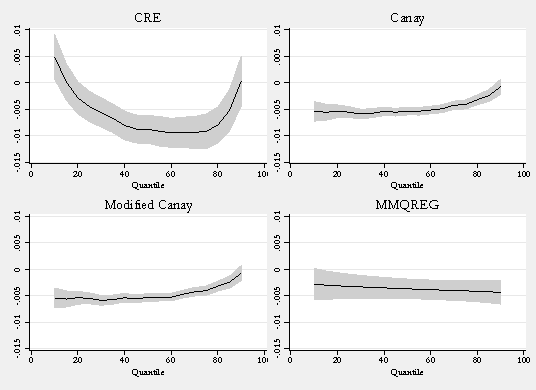
\includegraphics[width=1\textwidth,height=\textheight]{qregplot_age.pdf}

}

\caption{\label{fig-age}QR Coefficients for Age}

\end{figure}%

When considering Tenure, Figure~\ref{fig-tenure}, all estimators suggest
very similar results. As tenure increases, one would also expect higher
wages, with largest effects at the bottom of the distribution, but
decreasing as we move to the top. CRE results decline the least, while
Canay and Modified Canay show a steeper decline.

\begin{figure}[H]

\centering{

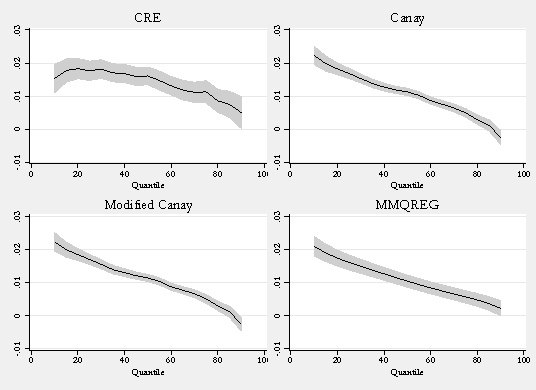
\includegraphics[width=1\textwidth,height=\textheight]{qregplot_tenure.pdf}

}

\caption{\label{fig-tenure}QR Coefficients for Tenure}

\end{figure}%

Finally, when considering experience, Figure~\ref{fig-ttl-exp}, the
results across estimators is mixed. They all suggest that, people with
more experience, also tend to earn higher wages, with the effect being
more pronounced the further up of the distribution we analyze. However,
the magnitude of the effect varies across estimators. CRE estimates
suggest the steppest change in this relationsip, with Canay and Modified
Canay suggesting a much flatter trend. MMQREG, on the other hand shows
results that are in between the other estimators.

\begin{figure}[H]

\centering{

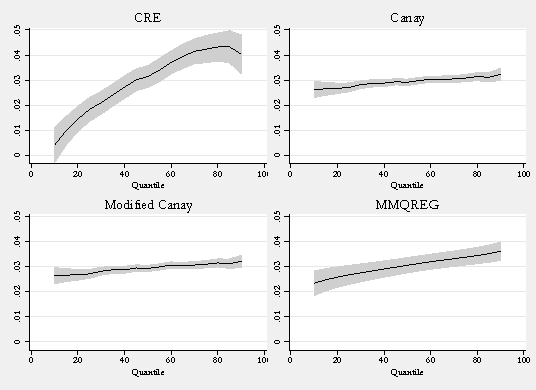
\includegraphics[width=1\textwidth,height=\textheight]{qregplot_ttl_exp.pdf}

}

\caption{\label{fig-ttl-exp}QR Coefficients for Experience}

\end{figure}%

\section{Conclusions}\label{sec:conclusions}

This paper has introduced two new Stata commands, \texttt{qregfe} and
\texttt{qregplot}, designed to estimate and visualize quantile
regression models with fixed effects. These commands address the growing
need for tools that can handle unobserved heterogeneity in quantile
regression frameworks, particularly in panel data settings.

The \texttt{qregfe} command offers an implementation of several
methodologies for estimating quantile regressions with fixed effects,
including the Correlated Random Effects (CRE) approach,
\citet{canay2011} estimator, a modified version of Canay's estimator,
and the Method of Moments Quantile Regression (MMQREG) proposed by
\citet{mss2019}. By providing these different estimation methods within
a single command, \texttt{qregfe} allows researchers to easily compare
results across methods and select the most appropriate approach for
their specific research context.

The companion command \texttt{qregplot} facilitates the visualization of
quantile regression results, enabling researchers to graphically examine
how the effects of covariates vary across different points of the
conditional distribution of the outcome variable. It can be used not
only with \texttt{qregfe}, but also with a large set of other quantile
regression commands. This type of visual representation is valuable for
identifying and interpreting heterogeneous effects that are harder to
observed simply using regression tables.

While these commands aim to make this methodologies more accessible to
applied researchers, it should be noted that each method relies on
specific assumptions that may not hold in all empirical settings. Thus,
one should carefully consider the underlying assumptions of each
approach and potentially compare results across methods to ensure robust
conclusions.

\clearpage

\bibliographystyle{sj}
\bibliography{bibliography.bib}


\begin{aboutauthors}

Fernando Rios-Avila is a Research Scholar at the Levy Economics
Institute of Bard College. Leonardo Siles is a master student at the
Universidad de Chile. Gustavo Canavire-Bacarreza is a Senior Economist
at the World Bank.

\end{aboutauthors}

\end{document}
